%%%%%%%%%%%%%%%%%%%%%%%%%%%%%%%%%%%%%%%%%
% Structured General Purpose Assignment
% LaTeX Template
%
% This template has been downloaded from:
% http://www.latextemplates.com
%
% Original author:
% Ted Pavlic (http://www.tedpavlic.com)
%
% Note:
% The \lipsum[#] commands throughout this template generate dummy text
% to fill the template out. These commands should all be removed when 
% writing assignment content.
%
%%%%%%%%%%%%%%%%%%%%%%%%%%%%%%%%%%%%%%%%%

%----------------------------------------------------------------------------------------
%	PACKAGES AND OTHER DOCUMENT CONFIGURATIONS
%----------------------------------------------------------------------------------------

\documentclass{article}

\usepackage{fancyhdr} % Required for custom headers
\usepackage{lastpage} % Required to determine the last page for the footer
\usepackage{extramarks} % Required for headers and footers
\usepackage{graphicx} % Required to insert images
\usepackage{latexsym}
\usepackage{mathtools}

\usepackage{lipsum} % Used for inserting dummy 'Lorem ipsum' text into the template


\usepackage{algorithm}
\usepackage{algorithmic}
\renewcommand{\algorithmicrequire}{\textbf{Input:}}
\renewcommand{\algorithmicensure}{\textbf{Output:}}
\newcommand{\algorithmicbreak}{\textbf{break}}
\newcommand{\algorithmicgiven}{\textbf{Given:}}
\newcommand{\BREAK}{\STATE \algorithmicbreak}
\newcommand{\GIVEN}{\STATEx \algorithmicgiven}

\usepackage{amsmath}

% Margins
\topmargin=-0.45in
\evensidemargin=0in
\oddsidemargin=0in
\textwidth=6.5in
\textheight=9.0in
\headsep=0.25in 

\linespread{1.1} % Line spacing

% Set up the header and footer
\pagestyle{fancy}
\lhead{\hmwkAuthorName} % Top left header
\chead{\hmwkClass\ : \hmwkTitle} % Top center header
\rhead{\firstxmark} % Top right header
\lfoot{\lastxmark} % Bottom left footer
\cfoot{} % Bottom center footer
\rfoot{Page\ \thepage\ of\ \pageref{LastPage}} % Bottom right footer
\renewcommand\headrulewidth{0.4pt} % Size of the header rule
\renewcommand\footrulewidth{0.4pt} % Size of the footer rule

\setlength\parindent{0pt} % Removes all indentation from paragraphs

%----------------------------------------------------------------------------------------
%	DOCUMENT STRUCTURE COMMANDS
%	Skip this unless you know what you're doing
%----------------------------------------------------------------------------------------

% Header and footer for when a page split occurs within a problem environment
\newcommand{\enterProblemHeader}[1]{
\nobreak\extramarks{#1}{#1 continued on next page\ldots}\nobreak
\nobreak\extramarks{#1 (continued)}{#1 continued on next page\ldots}\nobreak
}

% Header and footer for when a page split occurs between problem environments
\newcommand{\exitProblemHeader}[1]{
\nobreak\extramarks{#1 (continued)}{#1 continued on next page\ldots}\nobreak
\nobreak\extramarks{#1}{}\nobreak
}

\setcounter{secnumdepth}{0} % Removes default section numbers
\newcounter{homeworkProblemCounter} % Creates a counter to keep track of the number of problems

\newcommand{\homeworkProblemName}{}
\newenvironment{homeworkProblem}[1][Problem \arabic{homeworkProblemCounter}]{ % Makes a new environment called homeworkProblem which takes 1 argument (custom name) but the default is "Problem #"
\stepcounter{homeworkProblemCounter} % Increase counter for number of problems
\renewcommand{\homeworkProblemName}{#1} % Assign \homeworkProblemName the name of the problem
\section{\homeworkProblemName} % Make a section in the document with the custom problem count
\enterProblemHeader{\homeworkProblemName} % Header and footer within the environment
}{
\exitProblemHeader{\homeworkProblemName} % Header and footer after the environment
}

\newcommand{\problemAnswer}[1]{ % Defines the problem answer command with the content as the only argument
\noindent\framebox[\columnwidth][c]{\begin{minipage}{0.98\columnwidth}#1\end{minipage}} % Makes the box around the problem answer and puts the content inside
}

\newcommand{\homeworkSectionName}{}
\newenvironment{homeworkSection}[1]{ % New environment for sections within homework problems, takes 1 argument - the name of the section
\renewcommand{\homeworkSectionName}{#1} % Assign \homeworkSectionName to the name of the section from the environment argument
\subsection{\homeworkSectionName} % Make a subsection with the custom name of the subsection
\enterProblemHeader{\homeworkProblemName\ [\homeworkSectionName]} % Header and footer within the environment
}{
\enterProblemHeader{\homeworkProblemName} % Header and footer after the environment
}
   
%----------------------------------------------------------------------------------------
%	NAME AND CLASS SECTION
%----------------------------------------------------------------------------------------
\DeclarePairedDelimiter\ceil{\lceil}{\rceil}
\DeclarePairedDelimiter\floor{\lfloor}{\rfloor}
\newcommand{\hmwkTitle}{Homework\ \# 1 } % Assignment title
\newcommand{\hmwkDueDate}{Tuesday,\ March \ 10,\ 2015} % Due date
\newcommand{\hmwkClass}{MATH-578A} % Course/class
\newcommand{\hmwkClassTime}{11:00am} % Class/lecture time
\newcommand{\hmwkAuthorName}{Saket Choudhary} % Your name
\newcommand{\hmwkAuthorID}{2170058637} % Teacher/lecturer
%----------------------------------------------------------------------------------------
%	TITLE PAGE
%----------------------------------------------------------------------------------------

\title{
\vspace{2in}
\textmd{\textbf{\hmwkClass:\ \hmwkTitle}}\\
\normalsize\vspace{0.1in}\small{Due\ on\ \hmwkDueDate}\\
%\vspace{0.1in}\large{\textit{\hmwkClassTime}}
\vspace{3in}
}

\author{\textbf{\hmwkAuthorName} \\
	\textbf{\hmwkAuthorID}
	}
\date{} % Insert date here if you want it to appear below your name

%----------------------------------------------------------------------------------------

\begin{document}

\maketitle

%----------------------------------------------------------------------------------------
%	TABLE OF CONTENTS
%----------------------------------------------------------------------------------------

%\setcounter{tocdepth}{1} % Uncomment this line if you don't want subsections listed in the ToC

\newpage
\tableofcontents
\newpage




\begin{homeworkSection}{Question \# 1} % Section within problem

%\problemAnswer{
	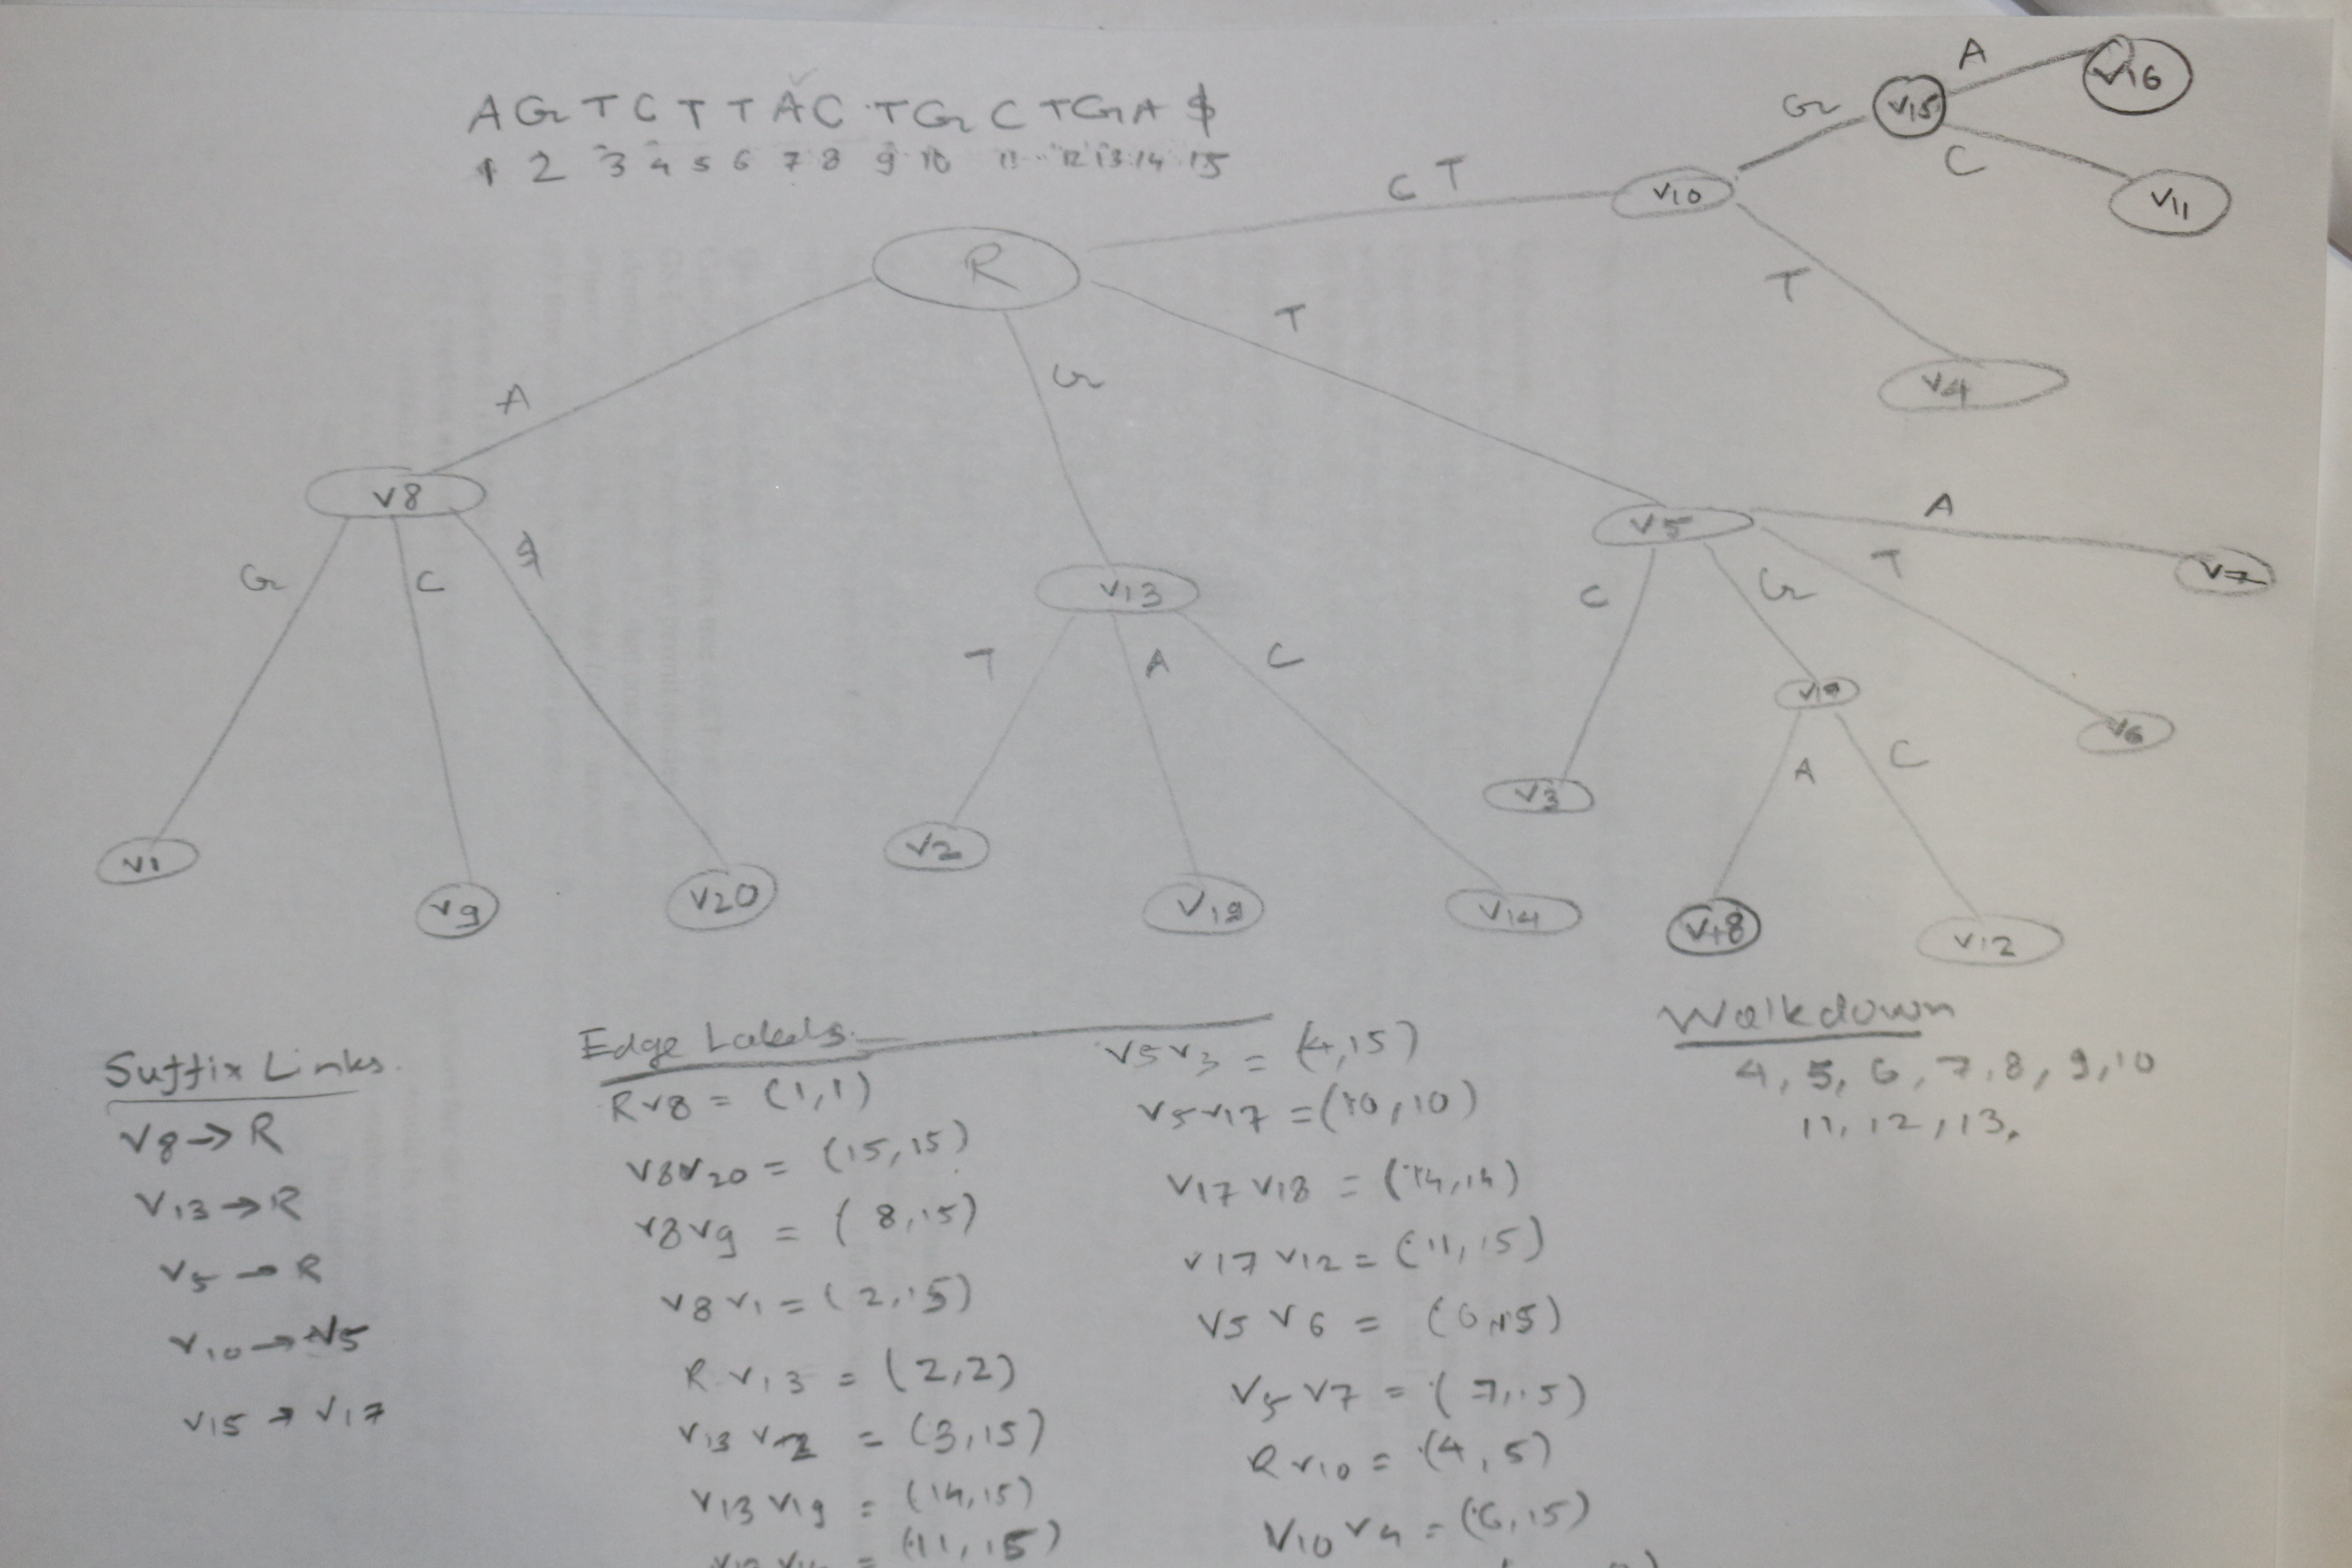
\includegraphics[width=\linewidth]{q1}
%}

\end{homeworkSection}

\begin{homeworkSection}{Question \# 2} % Section within problem

\problemAnswer{
	Space required to store the nodes of suffix tree : O(n)\\
	With edge label compression, each ege can be stored with two integers at each node denoting the start and end positions of the substring collapsed.\\
	Root: Stores nothing except at least two outgoing pointers. Each internal node stores 
	two $integers$ representing the start and end position so that the total size taken by each internal node is $2*sizeof(int)$
	Number of internal nodes = $n-1$. Hence total size occupied by nodes = $(n-1)*2*(sizeof(int*))$. The leaves store just one integer representing the start position of the suffix, so occupy $n*sizeof(int*)$ space. The edges are represented by pointers, so for a total of $2n-1$ nodes, there are $n-2$ edges for the internal nodes, each taking $sizeof(int*) + sizeof(int*)$ for representing the two integers at each node. Whike the pointers to the leaves takeup $n*sizeof(int*)$.
	In total:
		Internal nodes: $(n-1)*2*sizeof(int)$\\
		Leaves: $n*sizeof(int)$\\
		Internal Edges(Pointers): $(n-2)*sizeof(int*)$\\
		Terminal Edges(Pointers): $n*sizeof(int*)$\\
		Total = $3(n-1) * sizeof(int) + (2n-2)sizeof(int*)$ = $3(n-1)*(8)+(2n-2)*(64)= 136(n-1)$\\
		
	For a GST, on the leaves, we need to store the index of string that suffix came from, so an additional $n*(sizeof(int*))+n*(sizeof(int))$
, totaling $136(n-1)+64n+8n=208n-136$
		
	
	

}

\end{homeworkSection}


\begin{homeworkSection}{Question \# 3} % Section within problem

\problemAnswer{
	At each internal node store the identity of the leaves below it whether they come from $S_1, S_2...,S_k$ etc. This can be done
	using depth first traversal occupying $O(kn)$ space and $O(kn)$ in time.
	Since each internal node has atleast two children, the depth first traversal in a subtree is bounded by $O(kn)$.
	
	Construction of a GST is linear. It would require concatenating strings separated by unique delimiters(\$1\$2\$3...) and then
	follow suffix tree construction algorithm. Once the suffix tree has been constructed, a DFS from the root to leaves can then be used
	to store at each internal node which all string's suffixes are represented in the leaves below it. This is linear time too.
	The asymptotic space complexity is $O(kn)$ since each node can store at a maximum of $k+2$ values where $k$ represents number of different strings. Finding occurences of $P$ would involve tree traversal untill a fall off occurs at node $v$ after $m$ matches and the string ids stored at $v$ can be retrieved in constant time.
}

\end{homeworkSection}

\begin{homeworkSection}{Question \# 4} % Section within problem

\problemAnswer{
	We will assume $n$ is a  of type  $2^k-1$.
	 Make a $O(n)$ query for a LSB of the $n$ numbers. The number of $1$ and $0$ should ideally be same
	were all numbers present. Whichever occurence is smaller(0 or 1)($floor(\frac{N}{2}) )$, we do this for next $\frac{N}{2}$, then next $\frac{N}{4}$ and so on (total $O(2N)$) at each point storing which was lower $0 or 1$ and then recontruct the missing sequence.
	
	 Example:\\ 	$n=2^3-1=7$ so numbers from 0 to 7 should have been present. Let's say 5 is missing.
	 000\\
	 001\\
	 010\\
	 011\\
	 100\\
	 110\\
	 111\\
	 
	 First quesry on $7$ digits gives $4$ zeroes and $3$ ones. So LSB of missing number os $1$.
	 Now repeat for next significant bit for $3$ numbers:
	 001\\
	 111\\
	 111\\
	 
	 2 ones and 1 zeroes, so the next bit is $0$. Finally: 
	 001\\
	 1 zero and 0 ones. So missing bit is $1$
	 Missing number: 101
	 
}

\end{homeworkSection}

\begin{homeworkSection}{Question \# 5} % Section within problem

\problemAnswer{
	Hash table sizes are often prime numbers to minimise probability of collisions of unlike quantities. 
	Prime number modules ensures the number being divided go to maximum possible buckets(because the dividend and divisor will often be coprime).
	In the context of Rabin Karp, choosing a suitable prime is essential to prevent false positives, which would increase running time.
	
}

\end{homeworkSection}

\begin{homeworkSection}{Question \# 6} % Section within problem

\problemAnswer{
	Identifying longest substring starting at each position of T that occurs in P. 
    This requires creating a suffix tree for the pattern and not the text. Consider first m characters of text $T$
    and do a traversal of the suffix tree of pattern $P$. The last visited node's node edge depth will give the length 
    of longest substring match in $T[1..m]$ to some corresponding substring in $P$. Now consider finding sucha  substring
    that starts from position 2 of $T$ i.e $T[2..m]$ . This would now make use of the suffix link property. If the deepest possible
    visited during first step has path label $x\alpha$ then, the prefix of $T[2..m+1]$ is $\alpha$ which infact is just the suffix link 
    and this saves explicit character matches. Explicit matches are now performed from the suffix link node.
}

\end{homeworkSection}



\end{document}
